\documentclass[11pt]{article}
\usepackage[french]{babel}
\usepackage[utf8]{inputenc}
\usepackage[T1]{fontenc}
\usepackage[cm]{fullpage} % Rétraici les marges
\usepackage{amsmath}
\usepackage{amssymb}
\usepackage{graphicx}  % \includegraphics[scale=0.6]{image.png}\\
\usepackage{amsfonts} % Pour les ensembles IR, IN ...
\usepackage{tikz}

\title{Mathématique discrètes}
\date{2015-16, premier quadrimèstre}
\author{}

\begin{document}
\pagenumbering{Roman}
\maketitle
\tableofcontents
\pagebreak
\clearpage
\setcounter{page}{1}
\pagenumbering{arabic}

\section{Théorie des graphes:}
	\subsection{Définitions} 
		\subsubsection{Introduction}
	
			Un \textbf{graphe} $\Gamma$ est un triplet $(V,E,\gamma)$ où:
			\begin{itemize}
				\item $V$ est un ensemble fini dont les éléments sont appelés \textbf{sommets} ;
				\item $E$ est un ensemble fini dont les éléments sont appelés \textbf{arrêtes} ;
				\item $\gamma$ est une fonction qui associe à chaque arrête $e \in E$ une paire de sommets $\{x,y\} \in V$.
			\end{itemize}
			Qu'on notera plus généralement $\Gamma=(V,E)$
			
			\begin{minipage}{0.5\textwidth}
			\center  
			\begin{tikzpicture}
				\draw (0,2) node[anchor=south east]{$a$} node{\textbullet};
				\draw (0,1) node[anchor=east]{$b$} node{\textbullet};
				\draw (0,0) node[anchor=north east]{$c$} node{\textbullet};
				\draw (3,1) node[anchor=west]{$d$} node{\textbullet};
				\draw (0,0.5) ellipse (0.2 and 0.5);
				\draw (0,1.5) ellipse (0.2 and 0.5);
				\draw[color=red] (0,2) -- (3,1);
				\draw  (1.5,1.7) node[color=red] {$e_1$};
				\draw (0,1) -- (3,1);
				\draw  (1.5,0.25) node[color=blue] {$e_2$};
				\draw[color=blue] (0,0) -- (3,1);
			\end{tikzpicture} \\
			\end{minipage}\hfill
			\begin{minipage}{0.5\textwidth}
			\center
			$V = \{a,b,c,d\}$ \\
			$E = \{e_1, e_2, ...\}$ \\
			$\gamma(e_1)=\{a,d\}$ \\
			$\gamma(e_2)=\{c,d\}$\\
			\end{minipage}
			\begin{center}
			\textit{Exemple de graphe.} \\
			\end{center}

			Soit $\gamma(e)=\{x,y\}$ pour $e \in E, \{x, y\} \in V$. On dit que $x$ et $y$ sont \textbf{adjacents} et que $e$ est \textbf{incidente} à $x$ et $y$. \\
		
		\subsubsection{Cas particuliers d'arêtes}
			On appelle \textbf{arêtes multiples} toutes les arêtes incidentes à 2 mêmes points.\\
			Un \textbf{lacet} est une arête incidente à un seul point.
			\begin{center}
			\begin{tikzpicture}
				\draw (0,1) node[anchor=east]{$x$} node{\textbullet};
				\draw (2,1) node[anchor=west]{$y$} node{\textbullet};
				\draw (0,1)[color=red] .. controls (1,1.4)  .. (2,1);
				\draw (0,1)[color=blue] .. controls (1,0.6) .. (2,1);
				\draw (1,1.3) node[anchor=south,color=red]{$e_1$};
				\draw (1,0.7) node[anchor=north,color=blue]{$e_2$};
				
				\draw(3.5,0) -- (3.5, 2);		
				\draw (5,1.3) node[anchor=south]{$x$} node{\textbullet};
				\draw[color=red] (5,0.8) ellipse (0.2 and 0.5) node{$e$} ;
			\end{tikzpicture} \\
			\textit{Graphe avec arête multiple et graphe avec lacet.} \\
			\end{center}
		Un graphe est dit \textbf{simple} s'il ne contient pas d'arête multiple ni de lacet.
		
		\subsubsection{Degré d'un sommet}
			Le \textbf{degré} d'un sommet $v \in V$ est le nombre d'arêtes incidentes à $v$ (les lacets comptent pours 2 arêtes). On le note: $deg(v)$.\\
			
			\underline{Théorème:} Soit $\Gamma = (V,E)$, alors $\displaystyle \sum_{v \in V} deg(v) = 2\# E$. Autrement dit la somme des degrés de tout les sommets est égale au nombre d'arête $\times$2. Ce qui implique que la somme des degrés d'un graphe est toujours paire.\\
			
			\begin{minipage}{0.5\textwidth}
			\centering
			\begin{tikzpicture}
				\draw (0,1) -- (3,1);
				\draw (1,0) -- (1,2);
				\draw (2,0) -- (2,2);
				\draw[color=red] (0,1)node{\textbullet};
				\draw[color=blue] (1,1)node{\textbullet};
				\draw[color=red] (1,0)node{\textbullet};
				\draw[color=red] (1,2)node{\textbullet};
				\draw[color=blue] (2,1)node{\textbullet};
				\draw[color=red] (2,0)node{\textbullet};
				\draw[color=red] (2,2)node{\textbullet};
				\draw[color=red] (3,1)node{\textbullet};
			\end{tikzpicture} \\
			\end{minipage}\hfill
			\begin{minipage}{0.5\textwidth}
			\center
			7 arêtes\\
			2 sommets (bleu) de degré 4\\
			6 sommets (rouge) de degré 1\\
			$2 \times 4 + 6 \times 1 = 14 = 2 \times $ nombre d'arête totale
			\end{minipage}
			
		\subsubsection{Graphe complet}
			Le \textbf{graphe complet} $K_n$ est le graphe simple à $n$ sommets pour lequel chaque paire de sommet est relié par \textbf{une et une seule} arête. Autrement dit, les sommets sont tous adjacents entre-eux.
			\begin{center}
			\begin{tikzpicture}
				\draw(0,2)node{\textbullet};
				\draw (0,0) node[]{$K_1$};
				\draw(1,0) -- (1,2);
				
				\draw(2,2)node{\textbullet};
				\draw(2,1)node{\textbullet};
				\draw(2,2) -- (2,1);
				\draw (2,0) node[]{$K_2$};
				\draw(3,0) -- (3,2);

				\draw(3.5,1)node{\textbullet};
				\draw(4.5,1)node{\textbullet};
				\draw(4,2)node{\textbullet};
				\draw(4,2) -- (3.5,1) -- (4.5,1) -- (4,2);
				\draw (4,0) node[]{$K_3$};
				\draw(5,0) -- (5,2);
				
				\draw(5.5,1)node{\textbullet};
				\draw(6.5,1)node{\textbullet};
				\draw(6,2)node{\textbullet};
				\draw(6,1.4)node{\textbullet};
				\draw(6,2) -- (5.5,1) -- (6.5,1) -- (6,2) -- (6,1.4) -- (5.5,1);
				\draw(6,1.4) -- (6.5,1);
				\draw (6,0) node[]{$K_4$};
				\draw(7,0) -- (7,2);
				
				\draw(8,2)node{\textbullet};
				\draw(8.5,1.7)node{\textbullet};
				\draw(8.3,1.1)node{\textbullet};
				\draw(7.7,1.1)node{\textbullet};
				\draw(7.5,1.7)node{\textbullet};
				\draw(8,2) -- (8.5,1.7) -- (7.5,1.7) -- (8,2) -- (7.7,1.1) -- (7.5,1.7) -- (8.3,1.1) -- (7.7,1.1) -- (8.5,1.7) -- (8.3,1.1) -- (8,2);
				\draw (8,0) node[]{$K_5$};	
			\end{tikzpicture}
			\end{center}
			
		\subsubsection{Sous-graphes}
			Un graphe $\Gamma ' = (U,F)$ est un \textbf{sous-graphe} de $\Gamma = (V,E)$ si : \\
			$U\subseteq$ et $F \subseteq E$. On notera $\Gamma ' \leq \Gamma$
	
	\subsection{Chemins}
		\subsubsection{Definition}
			Soit $\Gamma=(V,E)$ et $v,w \in V$, un \textbf{chemin} de $v$ à $w$ de longueur $n$ est une séquence alternée de $(n+1)$ sommets $v_0,v_1,...,v_n$ et de $n$ arêtes $e_1,e_2,...,e_n$ de la forme : $(v_0,e_1,v_1,e_2,v_2,...,v_{n-1},e_n,v_n)$.\\
			
			Un chemin est \textbf{simple} si aucun sommet ne se répète, sauf peut-être celui de départ ou d'arrivée.\\
			
			\begin{minipage}{0.5\textwidth}
			\centering
			\begin{tikzpicture}
				\draw(0,0) node[anchor=north east]{$v_3$} node{\textbullet};
				\draw(0,1) node[anchor=south east]{$v_1$} node{\textbullet};
				\draw(3,1) node[anchor=south]{$v_2$} node{\textbullet};
				\draw(2,0) node[anchor=north]{$v_4$} node{\textbullet};
				\draw(4,0) node[anchor=west]{$v_5$} node{\textbullet};
				\draw (2,0) -- (0,0) -- (0,1) -- (3,1) --(2,0) -- (4,0);
				\draw(1.5,1)[anchor=south] node{$e_1$};
				\draw(2.5,0.4)[anchor=west] node{$e_2$};
				\draw(0,0.5)[anchor=east] node{$e_3$};
				\draw(1,0)[anchor=north] node{$e_4$};
				\draw(3,0)[anchor=north] node{$e_5$};
				\draw[color=red] (0,1) -- (3,1) --(2,0) -- (4,0);
			\end{tikzpicture} \\
			\end{minipage}\hfill
			\begin{minipage}{0.5\textwidth}
			\center
			$(v_1,e_1,v_2,e_2,v_4,e_5,v_5)$ est un chemin simple de longueur 3 entre $v_1$ et $v_5$
			\end{minipage}\\
			
		\underline{Remarque:} Dans un graphe simple on notera juste la suite des sommets (car il existe qu'un seul chemin les reliants). Avec l'exemple ci-dessus : $(v_1,v_2,v_4,v_5)$

		\subsubsection{Graphe connexe}
            		Un graphe $\Gamma=(V,E)$ est \textbf{connexe} si $\forall x,y \in V : \exists$ un chemin de $x$ à $y$.\\
            		
            		Soit $\Gamma = (V,E)$ un graphe et $x \in V$, la \textbf{composante connexe} de $\Gamma$ contenant $x$ est le sous-graphe $\Gamma'$ de $\Gamma$ dont les sommets et les arêtes sont contenues dans un chemin de $\Gamma$ démarrant en $x$.\\ % Besoin de reformulation plus claire --> phrase en tout cas correcte      ET vérifier si c'est gamma ou gamma' à la fin. --> fix'd
            		
            		\begin{minipage}{0.5\textwidth}
            			\centering
            			\begin{tikzpicture}
            				\draw(0,0) node{\textbullet};
            				\draw(1,0) node{\textbullet};	
            				\draw(3,2) node{\textbullet};	
            				\draw(1,2) node{\textbullet};
            				\draw(2,1) node{\textbullet};
            				\draw(0,0) -- (1,0) -- (1,2) -- (2,1) -- (3,2) -- (1,2);
            			\end{tikzpicture} \\
            			\textit{Graphe connexe.}
            			\end{minipage}\hfill
            			\begin{minipage}{0.5\textwidth}
            			\centering
            			\begin{tikzpicture}
            				\draw(0,0) node{\textbullet};
            				\draw(1,0) node{\textbullet};	
            				\draw(3,2) node{\textbullet};	
            				\draw(1,2) node{\textbullet};
            				\draw(2,1) node{\textbullet};
            				\draw(0,0) -- (1,0);
            				\draw(2,1) -- (3,2) -- (1,2);
            			\end{tikzpicture} \\
            			\textit{Graphe non-connexe avec 2 composantes connexes.}
            			\end{minipage}
			
		\subsubsection{Cycles}	
			Soit $\Gamma = (V,E)$ et $v \in V$, un \textbf{cycle} est un chemin allant de $v$ à $v$. Il est \textbf{simple} si on ne passe pas plusieurs fois sur le même sommet (à part $v$).\\
			\begin{minipage}{0.5\textwidth}
						\centering
						\begin{tikzpicture}
							\draw(0,1) node[anchor=east]{$v$} node{\textbullet};
							\draw(1,1) node{\textbullet};	
							\draw(2,1) node{\textbullet};
					\draw (0,1) .. controls (0.5,1.2)  .. (1,1);
					\draw (0,1.2)[color=red,->] .. controls (0.5,1.4)  .. (1,1.2);
					\draw (0,1) .. controls (0.5,0.8) .. (1,1);
					\draw (0,0.8)[color=red,<-] .. controls (0.5,0.6)  .. (0.95,0.8);
					\draw (2,1) .. controls (1.5,1.2)  .. (1,1);
					\draw (2,1.2)[color=red,<-] .. controls (1.5,1.4)  .. (1.05,1.2);
					\draw (2,1) .. controls (1.5,0.8) .. (1,1);
					\draw (2,0.8)[color=red,->] .. controls (1.5,0.6)  .. (1,0.8);
						\end{tikzpicture} \\
						\textit{Cycle non-simple.}
						\end{minipage}\hfill
						\begin{minipage}{0.5\textwidth}
						\centering
						\begin{tikzpicture}
							\draw(0,0) node[anchor=north east]{$v$} node{\textbullet};
							\draw(1,0) node{\textbullet};	
							\draw(0.5,1) node{\textbullet};	
							\draw(0,0) -- (1,0) -- (0.5,1) -- (0,0);
					\draw [color=red,->] (0,-0.2) -- (1,-0.2);
					\draw [color=red,->] (1.2,0) -- (0.7, 1);
					\draw [color=red,->] (0.3,1) -- (-0.2,-0);
						\end{tikzpicture} \\
						\textit{Cycle simple.}
						\end{minipage}
	\subsection{Arbres}
		\subsubsection{Définition}
					Un \textbf{arbre} est un graphe simple, connexe qui ne contient aucun cycle. Ses sommets de degré 1 sont appelés \textbf{feuilles}.
					
					\begin{center}
					\begin{tikzpicture}
						\draw(2,0)[color=red] node{\textbullet};	
						\draw(2,1) node{\textbullet};
						\draw(3,2)[color=red] node{\textbullet};
						\draw(1,2) node{\textbullet};
						\draw(1,3)[color=red] node{\textbullet};
						\draw(0.5,3)[color=red] node{\textbullet};
						\draw(1.5,3)[color=red] node{\textbullet};
						\draw(2,0) -- (2,1) -- (1,2) -- (0.5,3);
						\draw(1,2) -- (1,3);
						\draw(1,2) -- (1.5,3);
						\draw(2,1) -- (3,2);
					\end{tikzpicture} \\
					\textit{Exemple d'arbre (feuilles en rouge).}
					\end{center}
			
					Si $T$ est un arbre avec $p \geq 2$ sommets, alors $T$ contient au moins 2 feuilles.\\
						
					\underline{Théorème :} Soit $T$ un graphe simple à $p$ sommets, alors : \\ 
					$T$ est un arbre $\Leftrightarrow T$ a $(p-1)$ arêtes et aucun cycle $\Leftrightarrow T$ à $(p-1)$ arêtes et est connexe.
		\subsubsection{Arbre couvrant}
			Un \textbf{arbre couvrant} dans un graphe $\Gamma$ est un arbre qui est un sous-arbre de $\Gamma$ et qui contient tous les sommets de $\Gamma$.
			
			Il est utile entre autres pour résoudre le problème du voyageur de commerce.
	
	\subsection{Isomorphisme}
		2 graphes $\Gamma_1 = (V_1,E_1,\gamma_1)$ et $\Gamma_2 = (V_2,E_2,\gamma_2)$ sont \textbf{isomorphes} s'il existe une bijection $f : V_1 \rightarrow V_2$ et une bijection $g : E_1 \rightarrow E_2$ telles que $\forall e \in E_1$, $e$ est incident à $v, w \in V_1$ si et seulement si $g(e)$ est incident à $f(v), f(w) \in V_2$. On note cela : $\Gamma_1 \cong \Gamma_2$. \\ % fix'd
		Autrement dit, les graphes ont le même nombre de sommets et sont connectés de la même façon. Autrement dit, si les deux graphes venaient à être dessinés, alors il n'y aurait qu'à déplacer les sommets de l'un pour obtenir la copie conforme de l'autre.\\
		\begin{center}
		\begin{minipage}{0.5\textwidth}
			\begin{tikzpicture}
				\draw(0,0) node[anchor=north east]{$c$} node{\textbullet};
				\draw(2,0) node[anchor=north west]{$b$} node{\textbullet};
				\draw(1,2) node[anchor=south]{$a$} node{\textbullet};
				\draw(1,1) node[anchor=south]{$d$} node{\textbullet};
				\draw(0,0) -- (2,0) -- (1,1) -- (0,0) -- (1,2) -- (2,0);
				\draw(3,1) node{$\cong$};
				\draw(4,0) node[anchor=north east]{$c'$} node{\textbullet};
				\draw(4,2) node[anchor=south east]{$a'$} node{\textbullet};
				\draw(6,0) node[anchor=north west]{$b'$} node{\textbullet};
				\draw(6,2) node[anchor=south west]{$d'$} node{\textbullet};
				\draw(6,0) -- (4,0) -- (4,2) -- (6,0) -- (6,2) -- (4,0);
			\end{tikzpicture} \\
			\end{minipage}\hfill
			\begin{minipage}{0.5\textwidth}
			\center
			$f(a) = a'$ \\
			$f(b) = b'$ \\
			$f(c) = c'$ \\
			$f(d) = d'$ 
			\end{minipage}\\
			\textit{Exemple de graphes isomorphes.}
		\end{center}
		
		Pour prouver que 2 graphes sont isomorphe on montre la bijection de chaque sommet (il doit avoir le même degré dans le graphe isomorphe et être adjacent aux mêmes sommets).\\
		Inversement pour prouver que 2 graphes ne sont pas isomorphe, il nous suffit de trouver un sommet qui n'est pas dans une bijection.
	
	\subsection{Graphe Hamiltonien}
		Un \textbf{graphe hamiltonien} est un graphe possédant au moins un cycle passant par tous les sommets une et une seule fois. Ces cycles sont appelés \textbf{cycles hamiltoniens}.
		\begin{center}
			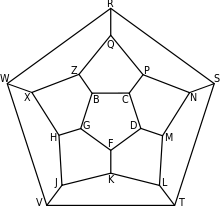
\includegraphics[scale=0.6]{hamiltonien.png}
			\qquad
			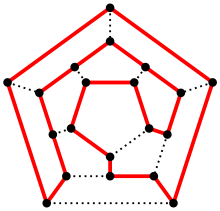
\includegraphics[scale=0.57]{hamiltonien2.png}\\
			\textit{Exemple de graphe hamiltonien et d'un cycle hamiltonien.}
		\end{center}
		
		Un graphe $\Gamma = (V,E)$ est \textbf{biparti} si on peut écrire $V = B \cup W$ avec $B \cap W = \emptyset$ et toute arête de $\Gamma$ joint un sommet de $B$ à un sommet de $W$. Avec $B$ et $W$ des sous-ensembles de sommets.
		\begin{center}
			\begin{tikzpicture}
				\draw (0,0)[color=red] ellipse (0.5 and 2);
				\draw (0,2)[color=red] node[anchor=south]{$B$};
				\draw (0,0) node{\textbullet};
				\draw (0,-0.75) node{\textbullet};
				\draw (0,0.75) node{\textbullet};
				\draw (0,-1.5) node{\textbullet};
				\draw (0,1.5) node{\textbullet};
				\draw (2,0)[color=blue] ellipse (0.5 and 1.25);
				\draw (2,1.5)[color=blue] node[anchor=south]{$W$};
				\draw (2,0) node{\textbullet};
				\draw (2,0.75) node{\textbullet};
				\draw (2,-0.75) node{\textbullet};
				\draw(0,0) -- (2,0.75);
				\draw(0,0) -- (2,-0.75);
				\draw(0,-0.75) -- (2,0.75);
				\draw(0,-1.5) -- (2,-0.75);
				\draw(0,-1.5) -- (2,0);
				\draw(0,0.75) -- (2,0.75);
				\draw(0,0.75) -- (2,-0.75);
				\draw(0,0.75) -- (2,0);
				\draw(0,1.5) -- (2,0.75);				
			\end{tikzpicture} \\
		\textit{Exemple de graphe biparti.}
		\end{center}
			
		Si un graphe est biparti, alors tout ses cycles simples sont de longueur paire.\\

		Un graphe biparti avec un nombre impair de sommets n'est pas hamiltonien. \\
		\begin{center}
			\begin{tikzpicture}
				\draw (0,0) node[anchor=south east, color=red]{$B$}node{\textbullet};
				\draw (1.5,0) node[anchor=south east, color=blue]{$W$}node{\textbullet};
				\draw (3,0) node[anchor=south east, color=red]{$B$}node{\textbullet};
				\draw (0,1.5) node[anchor=south east, color=blue]{$W$}node{\textbullet};
				\draw (1.5,1.5) node[anchor=south east, color=red]{$B$}node{\textbullet};
				\draw (3,1.5) node[anchor=south east, color=blue]{$W$}node{\textbullet};
				\draw (0,3) node[anchor=south east, color=red]{$B$}node{\textbullet};
				\draw (1.5,3) node[anchor=south east, color=blue]{$W$}node{\textbullet};
				\draw (3,3) node[anchor=south east, color=red]{$B$}node{\textbullet};	
				\draw (0,0) -- (3,0) -- (3,3) -- (0,3) -- (0,0);	
				\draw (1.5,0) -- (1.5,3);
				\draw (0,1.5) -- (3,1.5);	
			\end{tikzpicture} \\
		\textit{Exemple de graphe biparti non-hamiltonien.}
		\end{center}
		
		\underline{Théorème :} Soit $\Gamma$ un graphe simple avec $p \geq 3$ sommets et $\forall v \in V : deg(v) \geq \frac{1}{2}p$, alors $\Gamma$ est hamiltonien.
	
	\subsection{Illustration - Le code de Gray}
		Un code de Gray d'ordre $n$ est un arrangement cyclique de $2^n$ mots binaires de longueur $n$ tel que 2 mots ne différent qu'en une seule position.
		Par exemple pour $n=3$: \\ 
		\begin{minipage}{0.5\textwidth}
						\centering
						\begin{tikzpicture}
							\draw(0,1) node[anchor=east]{011} node{\textbullet};	
							\draw(1,0) node[anchor=north]{101} node{\textbullet};
					\draw(2,1) node[anchor=west]{110} node{\textbullet};
					\draw(1,2) node[anchor=south]{000} node{\textbullet};
					\draw(0.3, 1.71) node[anchor=south east]{001} node{\textbullet};
					\draw(0.3, 0.3) node[anchor=north east]{111} node{\textbullet};
					\draw(1.71, 0.3) node[anchor=north west]{100} node{\textbullet};
					\draw(1.71, 1.71) node[anchor=south west]{010} node{\textbullet};
					\draw(1,0) -- (1,2) -- (1.71,1.71) -- (0.3, 0.3) -- (1,0) -- (1.71,0.3) -- (0.3,1.71) -- (0,1) -- (2,1) -- (1.71,1.71);
					\draw(1,2) -- (0.3,1.71);
					\draw(2,1) -- (1.71,0.3);
					\draw(0,1) -- (0.3,0.3);
						\end{tikzpicture} \\
						\end{minipage}\hfill
						\begin{minipage}{0.5\textwidth}
						\centering
						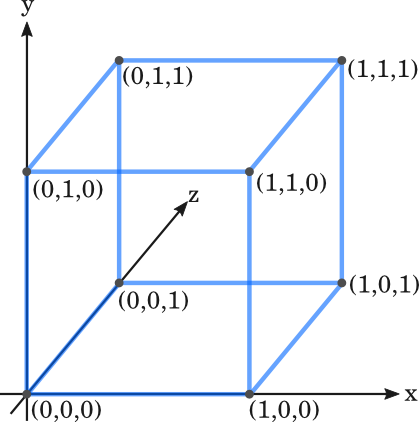
\includegraphics[scale=0.7]{cube_coords.png}
				\\
						\textit{Comparable aux sommets d'un cube.}
				\end{minipage}
		
	\subsection{Graphe Eulérien}
		Un \textbf{cycle eulérien} dans un graphe $\Gamma$ est un cycle qui contient toutes les arêtes de $\Gamma$. Un graphe est \textbf{eulérien} s'il contient un tel cycle.\\
		
		\underline{Proposition :} Si un graphe est eulérien, alors tout ses sommets sont de degré pair.\\
		
		\underline{Lemme :} Soit $\Gamma$ un graphe dans lequel chaque sommet est de degré pair, alors l'ensemble $E$ se partitionne\footnote{collection de sous-ensembles $C_1, ..., C_n$ de $E$ telle que $E=\displaystyle\bigcup^n_{i=1} C_i$ et $\forall i \neq j, C_i \cap C_j = \emptyset$.} en une union de cycles (arête-)disjoints.\\
		\begin{center}
			\begin{tikzpicture}
				\draw[color=blue](0,1) -- (1,0) -- (5,0) -- (6,1) -- (5,2) -- (1,2) -- (0,1);
				\draw[color=red](1,0) -- (2,1) -- (1,2) -- (1,0);
				\draw[color=teal](5,0) -- (5,2) -- (4,1) -- (5,0);
						\draw(0,1) node{\textbullet};
				\draw(1,0) node{\textbullet};
				\draw(2,1) node{\textbullet};
				\draw(1,2) node{\textbullet};	
				\draw(4,1) node{\textbullet};
				\draw(5,0) node{\textbullet};
				\draw(6,1) node{\textbullet};
				\draw(5,2) node{\textbullet};
						\end{tikzpicture} \\
				\textit{toutes les arêtes se trouvent dans un seul cycle.}
			\end{center} 
			
	\underline{Théorème :}  Soit $\Gamma$ un graphe connexe. $\Gamma$ est un graphe eulérien $\Leftrightarrow$ chaque sommet est de degré pair.

	\subsection{Ordre partiel}
		Soit $P$ un ensemble. Un \textbf{ordre partiel} sur $P$ est une relation sur $P$ (c'est-à-dire un ensemble de couples $(p_1,p_2) \in P \times P$) notée $p_1 \leq p_2$ telle que:
		\begin{itemize}
			\item Réflexivité : $p \leq p$ ;
			\item Anti-symétrie : $p \leq q$ et $q \leq p \Rightarrow p = q$ ;
			\item Transitivité : $p \leq q$ et $q \leq r \Rightarrow p \leq r$.
		\end{itemize}

		On note $(P,\leq)$ un ensemble partiellement ordonné.\\
		
		Un ordre partiel $(P,\leq)$ peut se représenter à l'aide d'un graphe. Si l'on place les arêtes entre les différents sommets en respectant les 3 règles d'un ordre partiel et en enlevant les arêtes pouvant être obtenues par transitivité, alors on obtient un \textbf{diagramme de Hasse}. C'est à dire le graphe simple $\Gamma = (P,E)$ tel que :
		\begin{itemize}
			\item $e = \{x,y\} \in E \Leftrightarrow x \leq y$ et $\not \exists z | (x \leq z) \land (z \leq y)$ ;
			\item Dans sa représentation : si $x \leq y, x$ sera placé plus bas que $y$.

		\end{itemize}
		
		\begin{center}
		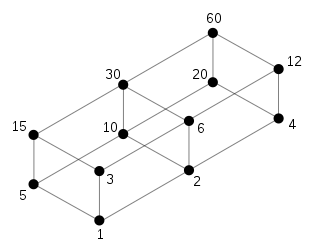
\includegraphics[scale=0.65]{ordre_partiel.png}\\
		\textit{Diagramme de Hasse de l'ensemble des diviseurs de 60, $A = \{1, 2, 3, 4, 5, 6, 10, 12, 15, 20, 30, 60\}$, ordonnés par la relation de divisibilité.}
		\end{center}
		
		Soit  $(P, \leq)$ un ordre partiel:
		\begin{itemize}
			\item Une \textbf{chaine} dans $P$ est un sous-ensemble $C$ de $P$ tel que :\\
			$\forall c_1,c_2 \in C : c_1 \leq c_2$ ou $c_2 \leq c_1$.\\
			(Dans l'exemple ci-dessus : $\{1,2,4,20,60\}$ en est une (1 divise 2, qui divisent 4, qui divisent 20, qui divisent  60)).
			\item Une \textbf{antichaîne} dans $P$ est un sous-ensemble $A$ de $P$ tel que :\\
			$\forall a_1 \neq a_2 \in A : a_1 \not\leq a_2$ et $a_2 \not\leq a_1$. Autrement dit c'est une partie dont les éléments sont 2 à 2 incomparables.
			(Dans l'exemple ci-dessus : $\{5,3,2\}$ en est une (5 ne divise pas 3 et 3 ne divise pas 2)).\\
		\end{itemize}
		
		\underline{Théorème (Dilworth):} Soit $(P,\leq)$ un ensemble fini partiellement ordonné. Alors $\exists$ une antichaine $A$ une partition de $P$ par des chaînes $Q=\{C_1,C_2,...,C_n\}$ tels que $\#Q=\#A$. Autrement dit, le théorème de Dilworth établit, pour un ordre fini, l'existence d'une antichaîne $A$ et d'une partition de l'ensemble ordonné en une famille $Q$ de chaînes, telles que $A$ et $Q$ aient même cardinal.\\
		
		\underline{Remarques :}
		\begin{itemize}
			\item $Q$ une partition de $P$ et $A$ une antichaîne dans $P$ alors $\#A \leq \#Q$ ;
			\item $(P,\leq)$ ordre total. Alors une antichaîne non-vide a exactement 1 élément.
		\end{itemize}

		\underline{Lien avec les graphes bipartis :}
		
		Soit $\Gamma=(V,E)$ un graphe simple; un \textbf{couplage} $M$ de $\Gamma$ est un sous-ensemble d'arêtes de $E$ qui sont 2 à 2 non-adjacentes. Les sommets incidents aux arêtes de $M$ sont dits couplés. Autrement dit, c'est un ensemble d'arêtes qui n'ont pas de sommets en commun.\\
		
		Un \textbf{transversal} de $\Gamma$ est un sous-ensemble $T$ de sommets de $V$ tel que toute arête de $E$ est incidente à au moins 1 sommet de $T$.\\
			
		\begin{minipage}{0.5\textwidth}
					\centering
						\begin{tikzpicture}
					\draw[color=blue](1.5,0)--(0,0)--(1.5,1);
					\draw[color=blue](1.5,2)--(0,2);
					\draw[color=blue](1.5,4)--(0,3);
					\draw[color=blue](1.5,3)--(0,4);
					\draw(1.5,3)--(0,3);
					
							\draw(0,0)[color=red] node{\textbullet};
					\draw(0,2) node{\textbullet};	
					\draw(0,3) node{\textbullet};
					\draw(0,4) node{\textbullet};
					\draw(1.5,0) node{\textbullet};
					\draw(1.5,1) node{\textbullet};
					\draw(1.5,2)[color=red]  node{\textbullet};
					\draw(1.5,3)[color=red]  node{\textbullet};
					\draw(1.5,4)[color=red]  node{\textbullet};
						\end{tikzpicture}
						\end{minipage}\hfill
						\begin{minipage}{0.5\textwidth}
						\centering
				\textit{En rouge : transversal à 4 sommets,\\
						en bleu : couplage à 4 arêtes}
				\end{minipage}\\

		\underline{Théorème (König):} Soit $\Gamma = (V= B\ \amalg\ W\footnote{$B \cup W = V$ et $B \cap W = \emptyset$}, E)$ un graphe biparti. Alors la cardinalité maximale d'un couplage de $\Gamma$ est égale à la cardinalité minimale d'un transversal de $\Gamma$.\\
		
		Soit $\Gamma=(B \amalg W,E)$ un graphe biparti et $M$ un couplage. Un \textbf{chemin alterné} est un chemin qui démarre en un sommet de $B$ non-couplé et alterne une arête dans $E \setminus M$ puis une arête dans $M$ et ainsi de suite.
		\begin{center}
			\begin{tikzpicture}
				\draw(0,0) node[anchor=east]{$b_5$} node{\textbullet};
				\draw(0,1) node[anchor=east]{$b_4$}  node{\textbullet};	
				\draw(0,2) node[anchor=east]{$b_3$}  node{\textbullet};	
				\draw(0,3) node[anchor=east]{$b_2$}  node{\textbullet};
				\draw(0,4) node[anchor=east]{$b_1$}  node{\textbullet};
				\draw(2,0) node[anchor=west]{$w_4$} node{\textbullet};
				\draw(2,1) node[anchor=west]{$w_3$} node{\textbullet};
				\draw(2,2) node[anchor=west]{$w_2$} node{\textbullet};
				\draw(2,3) node[anchor=west]{$w_1$} node{\textbullet};
				\draw(0,0) -- (2,0) -- (0,1) -- (2,1) -- (0,2) -- (2,2) -- (0,3) -- (2,3) -- (0,4);
					\end{tikzpicture}\\
			\textit{Exemple de chemin alterné}
		\end{center}

		\underline{Proposition :} Le théorème de König est équivalent au théorème de Dilworth.



\section{Arithmétique modulaire et introduction aux graphes et anneaux}
	\subsection{Les entiers et la division euclidienne}
		\subsubsection{Les entiers}
			L'ensemble des entiers est noté $\mathbb Z$, il contient les entiers naturels ($\mathbb N$) et leurs opposé.\\
			Cet ensemble est régi par 2 opérations:
			\begin{itemize}
				\item L'addition usuelle dans $\mathbb Z : + \mathbb Z \times \mathbb Z \rightarrow \mathbb Z : (a,b) \mapsto a+b$\\
				Propriétés:
				\begin{enumerate}
					\item est commutative $\Leftrightarrow a + b = b + a$
					\item est associative $\Leftrightarrow a + (b + c) = (a + b) + c$
					\item admet un élément neutre noté $0 \Leftrightarrow 0 + a = a$
					\item admet un opposé noté $-a \Leftrightarrow a + (-a) = 0$
				\end{enumerate}
				On dit que ($\mathbb Z$, +) est un groupe (2,3,4) commutatif (1).

				\item Multiplication: $\cdot: \mathbb Z\times Z \to Z : (a,b) \mapsto a \cdot b$\\
				Propriétés:
					\begin{enumerate}
						\item est associative: $a\cdot(b\cdot c) = (a \cdot b) \cdot c$
						\item est distributive par rapport à l'addition : $a \cdot (b + c) = a\cdot b + a \cdot c$ et $(a+b)\cdot c = ac +bc$
						\item est commutative : $a \cdot b = b \cdot a$
						\item $a \cdot b = a \cdot c \Leftrightarrow c = b$
						\item admet un neutre : $1 \in \mathbb Z, 1 \cdot a = a = a \cdot 1$
					\end{enumerate}
			\end{itemize}
			On dit que $(\mathbb Z, + , \cdot)$ est un anneau \footnote{$(\mathbb Z,+)$ est un groupe commutatif, satisfait propriétée 1 et 2} unital\footnote{propriétée 5}, commutatif\footnote{propriétée 3} et intègre\footnote{propriétée 4}.\\

			On à sur $\mathbb Z$, une relation d'ordre $\leq$ tels que:
			\begin{enumerate}
				\item $\leq$ est un ordre total
				\item $a \leq b \Rightarrow a+c \leq b + c$
				\item $a \leq b, c \geq 0 \Rightarrow a \cdot c \leq b \cdot c$
			\end{enumerate}

		\subsubsection{La division euclidienne}
			L'équation $a \cdot x = b$ avec $a, b \in \mathbb Z$, n'a pas toujours de solutions dans $\mathbb Z$.\\
			Soir $a, b \in \mathbb Z$, on dit que $a$ divise $b$ et on note $a/b$, si $\exists c \in \mathbb Z | a \cdot c = b$. $/$ est une relation.\\
			Propritétés:
			\begin{enumerate}
				\item Réflexion : $a/a$
				\item transitivité : $a/b$ et $b/c \Rightarrow a/c$
				\item Anti-symétrique : $a/b$ et $b/a \Rightarrow a = \pm b$ 
			\end{enumerate}
			\underline{Théorème (\textbf{Division Euclidienne}) :} $\forall a, b \in \mathbb Z, b \neq 0, \exists$ des entiers uniques $q$ (quotient), $r$ (reste) tel que $a = b \cdot q + r$ et $0 \leq r < |b|$\\

			Un nombre $p \in \mathbb Z$ est premier si $p \neq -1, 1, 0$ et $p$ n'est divisible que par $1, -1, p$ et $-p$.\\

			Un entier $d$ est un plus grand commun diviseur de 2 entier non nuls $a$ et $b$ si et seulement si:
			\begin{itemize}
				\item $d / a$ et $d / b$
				\item $c \in c / a$ et $c / b \Rightarrow c / d$
			\end{itemize}
			On note $pgcd(a, b)$ le plus grand commun diviseur positif de $a$ et $b \in \mathbb Z_0$ et on pose $pgcd(a, 0) = |a| \forall a \in Z$\\

			\underline{L'algorithme d'Euclide :} Si $a, b \in \mathbb Z, b \neq 0$, soit $q, r, \in \mathbb Z : a = b \cdot q + r$  alors $pgcd(a, b) = pgcd(b, r)$.\\
			Pour calculer le $pgcd(a, b) \forall a, b \in \mathbb Z, b \neq 0$ on procède comme suit :\\
			On peut supposer que $a$ et $b \geq 0$ car $pgcd(a, b) = pgcd(-a, b) = pgcd(a, -b) = pgcd(-a, -b)$\\
			Par le théorème de la division euclidienne :
			\begin{itemize}
				\item $a = b \cdot q_1 + r_1$ pour $q_1 \in \mathbb Z, 0 \leq r_1 < b$
				\item $\Rightarrow pgcd(a, b) = pgcd(b, r_1)$
				\item Si $r_1 = 0 : pgcd(a, b) = pgcd(b, 0) = b$
				\item Sinon $r_1 > 0 :$ on itère : $b = r_1 \cdot q_1 + r_2  pour q_2 \in \mathbb Z, 0 \leq r_2 < r_1$
				\item $\Rightarrow pgcd(b, r_1) = pgcd(r_1, r_2)$
				\item On itère pour obtenir des restes $r_1 > r_2 > r_3 > … > r_n > r_{n+1} = 0$
				\item On a $pgcd(a, b) = pgcd(b, r_1) = pgcd(r_1, r_2) = … = pgcd(r_n-1, r_n) = pgcd(r_n, r_{n+1} (=0) ) = r_n$
			\end{itemize} 
			\begin{center}
				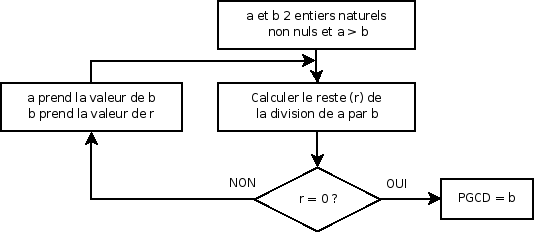
\includegraphics[scale=0.6]{Algorithme_PGCD.png}
			\end{center}

			Soient $a, b \in \mathbb Z, b \neq 0, alors \exists s, t \in \mathbb Z : pgcd(a, b) = s \cdot a + t \cdot b$\\
			Exemple ; $pgcd(51,42)$:
			\begin{align*}
				51 &= 42 \cdot 1 + 9\\
				42 &= 9 \cdot 4 + 1\\
				9 &= 6 \cdot 1 + 3\\
				6 &= 3 \cdot 2\\
				pgcd(51,42) &= 3
			\end{align*}
			Trouvons $s$ et $t$ tel que $s \cdot 51 + t \cdot 42 = 3$
			\begin{align*}
				s_1 = 1\quad & t_1 = -1\\
				s_2 = -1\quad & t_2 = 1 - (-1) \cdot 4 = 5\\
				s_3 = 5\quad & t_3 = -1 - 5 \cdot 1 = -6\\
				5 \cdot 51 + (-6) \cdot 42 &= 3
			\end{align*}

			\underline{Décomposition en facteurs premiers:}\\
			2 nombres entiers non-nuls $a$ et $b$ sont premiers entre eux (ou relativement premiers) si $pgcd(a, b) = 1$.\\

			\underline{Proposition (de Bézout) :} Deux entiers $a$ et $b$ sont premiers entre eux si et seulement si $\exists s, t \in \mathbb Z$ tel que $s \cdot a + t \cdot b = 1$\\

			\underline{Proposition (de Gauss) :} Si $a$ et $b$ sont premiers entre eux et $c \in \mathbb Z$ tel que $b / a \cdot c \Rightarrow b / c$\\
			Corrolaire : Si $p$ est premier et $p /ab$, avec $a,b \in \mathbb Z \Rightarrow p/a$ ou $p/b$.\\

			\underline{Théorème (Factorisation) :} $\forall $entier$ z \in \mathbb Z_0, \exists n \in \mathbb N, \exists p_1, …, p_n$ des nombres premiers positifs deux à deux différents et $\exists e_1, …, e_n \in N_0$ tel que :\\
			$z = (\pm 1) p_1^{e_1}, p_2^{e_2}, …, p_n^{e_n}$\\
			Cette expression est unique à l'ordre dans lequel on écrit $p_i^{e_i}$ près.
			
  
	\subsection{Groupes, anneaux et entiers modulo $h$}
		\subsubsection{Définition}
			Un groupe $(G,*)$ est un ensemble non-vide $G$ muni d'une loi de composition 
			\begin{align*}
				* :&\ G \times G \rightarrow G\\
				&\ (g,h) \mapsto g * h
			\end{align*}
			tels que :
			\begin{enumerate}
				\item $*$ est associatif : $\forall g,h,k \in G : (g * h) * k = g * (h * k)$
				\item $\exists$ un neutre $e \in G : g * e = g = e * g \qquad \forall g \in G$
				\item $\forall g \in G : \exists$ un inverse $g^{-1} \in G$ tel que $g * g^{-1} = e = g^{-1}  g$
			\end{enumerate}

			Par exemple :
			\begin{itemize}
				\item $(\mathbb Z, +) \rightarrow$ groupe
				\item $(\mathbb Z_0, \cdot) \rightarrow$ pas un groupe (3. pas respecté, ex: $2^{-1} = \frac{1}{2} \not\in \mathbb Z$)
				\item $(\mathbb R, \cdot) \rightarrow$ pas un groupe (3.  pas respecté, car 0 n'a pas d'inverse ; $0 \cdot x = 0 \neq e = 1$)
				\item $(\mathbb R_0, \cdot) \rightarrow$ un groupe
				\item $V$ espace vectoriel $\rightarrow$ groupe
				\item $(Gl(V) = \{f : V \rightarrow V \setminus f$ isomorphisme linéaire $\}, 0) \rightarrow$ groupe
				\item $(Gl2(\mathbb R) = \{
					\begin{pmatrix}
  						a_1 & b_1 \\
						a_2 & b_2 
					\end{pmatrix} 
					| a, b, c, d \in \mathbb R  a \cdot d – b \cdot c \neq 0\}, \cdot) \rightarrow$ groupe
			\end{itemize}
			
			
			\underline{Définition :} Soit $(G, *)$ un graphe. Un sous ensemble $H$ de $G$ est un sous-graphe de $G$ si $(H,*)$ est un graphe. On note $(H,*) \leq (G,*)$ ou bien $H \leq G$\\
			
			\underline{Proposition :} $(G, *)$ un groupe et $H \in G$ \\
$H$ est un sous-groupe de $G$ si et seulement si :
			\begin{enumerate}
				\item $e \in H$
				\item $\forall g,h \in H : g * h^{-1} \in H$
			\end{enumerate} 
			Exemple : Dans $(\mathbb Z, +), 2 \mathbb Z = \{ ..., -2, 0, 2, ... \} = \{2z | z \in \mathbb Z \}$\\
			
			\underline{Proposition :} Soit $S \in \mathbb Z$  un sous-ensemble non-vide de $\mathbb Z$  tel que $(S, +) \leq (\mathbb Z , +) \Rightarrow \exists k \in\mathbb Z  : S = k\mathbb Z$\\
			
			Exemple :  Interprétation du $pgcd$: \\
$k, l \in\mathbb Z$  on définit $k \mathbb Z  + l \mathbb Z  =\{ k \mathbb Z 1 + l \mathbb Z 2 | \mathbb Z 1, \mathbb Z 2 \in\mathbb Z \}$
si $l \neq : k \mathbb Z  + l \mathbb Z  = pgcd(k, l) \mathbb Z$

		\subsection{Groupes quotients}
			Dans cette section, on considère $(G, +)$ un groupe commutatif.  Dans ce cas, l'inverse de $g \in G$ se note $-g$ on l'appelle aussi l'opposé de $g$.\\
			
			\underline{Définition :} Soit $(H, +) \leq (G +)$. Une \textbf{classe latérale} de $H$ est un ensemble :
$g+H = \{ g+h | h \in H \}$ pour un $g \in G$ fixé\\
			\underline{Proposition : } $(H, +) \leq (G, +), g, g'  \in G : g+H = g' + H <=> \forall h \in H, \exists!\footnote{Il existe un unique}\  h' \in H : g + h = g' + h'.$\\
			
			\underline{Définition :} On notre $G/H$ l'ensemble des classes latérales de $H$, pour $(H, +) \leq (G, +)$ \\
$G/H = \{ g+h | g \in G \} \qquad g + h$ seras noté $\overline{g}$ \\
			Exemple : $(\mathbb Z , +)$ et $7 \in\mathbb Z  : 
\mathbb Z  / 7\mathbb Z  = {0 + 7\mathbb Z , 1+7\mathbb Z , 2+7\mathbb Z , …, 6+7\mathbb Z }
= \{ \overline{0}, \overline{1}, \overline{2}, \overline{3}, \overline{4}, \overline{5}, \overline{6} \}$\\
			
			Division euclidienne : $\forall \mathbb Z  \in\mathbb Z  : \exists r tel quel : \mathbb Z  = 7q + r => \mathbb Z  \in \overline{z} = r + 7\mathbb Z$\\
			 
			\underline{Proposition :} $ (\mathbb Z , +)$ et $k \in\mathbb Z$  alors $\mathbb Z  / k \mathbb Z$  est une partition de $\mathbb Z $
			
			\underline{Théorème :} Soit $(G, +)$ un groupe (commutatif) et $H \leq G$
Alors $G/H$ est muni d'une loi $\mp$ tel que $(G/H, \mp)$ est un groupe commutatif.  Précisément, on définit :
$\forall g, g' \in G : \overline{g} \mp \overline{g'} := \overline{(g+g')}$\\
ou bien $(g+H) \mp (g'+H) := (g+g') + H$
			\underline{Démonstration :} Montrons que I est bien défini:\\
			$g, \tilde{g}, g', \tilde{g'} \in G : \overline{g} = \overline{\tilde{g}}$ et $\overline{g'} = \overline{\tilde{g'}}$\\
			Montrons que $\overline{g} \overline{+} \overline{g'} = \overline{\tilde{g}} \overline{+} \overline{\tilde{g'}}$\\
			$\overline{g} = \overline{\tilde{g}} \Rightarrow g + (-\tilde{g}) = h \in H, \overline{g'} = \overline{\tilde{g'}} \Rightarrow g' + (\tilde{g'}) = h' \in H$
			
			$\overline{g} \overline{+} \overline{g'} = \overline{g+g'} = ((\tilde{g}+h) + \overline{\tilde{g'} + h')} = (\tilde{g} + \tilde{g'} + \overline{h + h'}$
			et (c'est égal à) $\overline{\tilde{g}} \overline{+} \overline{\tilde{g'}} = \overline{\tilde{g}+\tilde{g'}}$
			
			\begin{itemize}
			 \item $\overline{+}$ est associatif, commutatif : on les récupère des propriété de +
			 \item $g \in G : -\overline{g} = -(g+H) := (-g) + H = -\overline{g}$
			 \item $e \in G$ alors $\overline{e} \in G/$H est le neutre pour I
			\end{itemize}

			\underline{Définition (Exemple principal de groupe quotient) :} Pour $n \in N_0, n Z \leq Z$, on définit le groupe des entiers modulo $n$ comme le groupe quotient $(Z/nZ, I) $où$ \overline{a} \overline{+} \overline{b} = \overline{a+b} \forall a, b \in Z$
			
			\underline{Exemple :} $Z/8Z = {\overline{0}, \overline{1}, \overline{2}, \overline{3}, \overline{4}, \overline{5}, \overline{6}, \overline{7}}, \overline{2} \mp \overline{5} = \overline{7}, \overline{6} \overline{+} \overline{7} = \overline{13} = \overline{5}$\\
				$\overline{0}$ est le neutre: $\overline{4} + \overline{0} = \overline{4+0} = \overline{4}$\\
				L'opposé: $- \overline 3 = \overline{-3} = \overline{5}$
		
		\subsection{Isomorphisme de groupes}
			\subsubsection{Définition}
				Soient $(G, *)$ et $(G', *')$ deux groupes. Un morphisme de groupe est une application f: G -> G' tel que $\forall g, h \in G: f(g*h) = f(g) *' f(h)$\\
				Exemple : 
				\begin{itemize}
					\item $(R, +)$ et $(R_0 +, .)$\\
					Exponentiel: $R \rightarrow R_0^+ : x \mapsto e^x$ morphisme car $\forall x, y \in R : e^{x+y} = e^x \cdot e^y$
					 \item Logarithme: $R_0^+ \rightarrow R$\\
					Morphisme: $log(x, y) = log(x) + log(y)$
				 	\item $Z, p: Z \rightarrow Z/kZ : z \mapsto \overline{z}$ morphisme surjectif mais pas injectif.
					 \item $(Z/8Z, +)$ et $(R_4, .)$ racine 4ème de l'unité dans C (complexe)\\
					$f: Z/8Z \rightarrow R_4 : \overline{l} \mapsto e^((2\pi i 2l )/8)$ morphisqme surjectif mais pas injectif
					 \item $(Gl_2(R), \cdot ) et (R_0, \cdot )$ \\
					dét : $G\overline{l}2(R) \rightarrow R_0 : 
						\begin{pmatrix}
  							a & b \\
							c & d 
						\end{pmatrix}
						\mapsto ad - bc$ est un morphisme de groupe.
				\end{itemize}
	
			\underline{Définition :} Un morphisme de groupe $f: G \rightarrow G'$ est dit:
			\begin{itemize}
				\item \textbf{injectif} : si $\forall g1, g2 \in G: f(g1) = f(g2) \Rightarrow g1 = g2$
				\item \textbf{surjectif} : si $\forall g' \in G': \exists g \in G$ tel que $f(g) = g'$\\
			\end{itemize}
			
			\underline{Définition :} Soient $(G, *)$ et $(G', *')$ 2 groupe et $f:G \rightarrow G'$ un morphisme de groupe:
			\begin{itemize}
				\item L'image de f est l'ensemble: $Im(f) = \{ f(g) | g \in G\} \subseteq G$
				\item Le noyau de $f$ est l'ensemble : $Ker(f) = \{ g \in G | f(g) = e'  \} \subseteq G$
			\end{itemize}
			\underline{Propriété :} 
			\begin{itemize}
				\item $Ker(f)$ est un sous-groupe de G
				\item $Im(f)$ est un sous-graoupe de G'.
			\end{itemize}
			Exemple (en reprenant ceux plus haut): 
			\begin{itemize}
				\item[3] $p: Z -> Z/kZ$//
					$l-> \overline{l}$
					$Ker(p) = kZ \leq K$
				\item[4] $Ker(f) = \{\overline{0}, \overline{4}\} \leq Z/8Z$
				\item[5] $Ker(det) = \{
				\begin{pmatrix}
  					a & b \\
					c & d 
				\end{pmatrix}
				 a, b, c, d \in \mathbb R$ tel que $det(
				\begin{pmatrix}
  					a & b \\
					c & d 
				\end{pmatrix}) = 1\} S\overline{l}2(\mathbb R)$
			\end{itemize}
			\underline{Propriété :} Soient $(G, *)$ et $(G', *')$ deux groupes et $f: G \rightarrow G'$ un morphisme de groupe. Alors:
		 	\begin{enumerate}
				\item $f$ est injectif $\Leftrightarrow Ker(f) = \{e\}$
				\item $f$ est surjectif $\Leftrightarrow Im(f) = G'$
			\end{enumerate}
			\underline{Démonstration :}
			\begin{enumerate}
				\item $\left[ \Rightarrow \right]$
				\begin{itemize}
					\item  Montrons que $e \in Ker(f)$: $f(e) = f(e*e) = f(e) *' f(e)$\\
					$\Rightarrow f(e) = f(e) *' f(e) \Rightarrow f(e) = e'$\\
					Or dans un groupe $(F', *')$ si $x \in G': x *' x = x \Rightarrow x = e'$\\
					$\rightarrow x *' x = x \Leftrightarrow x *' x *' x^-1 = x * x^-1 = x *' e' = e' \Leftrightarrow x = e'$
					\item $\forall g \in Ker(f): f(g) = e' = f(e) \Rightarrow g = e$
					$\Rightarrow Ker(f) = {e}$
				\end{itemize}
					\item $\left[ \Leftarrow \right]$ Exercice
			\end{enumerate}
			
				Montrons que f est injectif
				$g1, g2 \in G: f(g1) = f(g2)$
		$\Leftrightarrow f(g1) *' (f(g2))^-1 = f(g2) *' (f(g2))^1 = e'$ \\
		Or si $x \in G: (f(x))^-1 = f(x^-1)$ \\
			$f(x^-1) *' = f(x^-1 * x) = f(e) = e'$ \\
			$\Rightarrow f(x^-1) = (f(x))^-1$
			
			$e' = f(g1) *' (f(g2))^-1$
			$= f(g1) * f(g2^-1)$
			$= f(g1 * g2^-1)$
			$\Rightarrow g1 * g2^-1 \in Ker(f) = par hypothèse {e} \in g1 * g2^-1 = e \Rightarrow g1 = g2$\\
			
			\underline{Définition :} Soient $(G, *)$ et $(G', *')$ 2 groupes
				\begin{itemize}
		 			\item Un \textbf{isomorphisme} de groupe est un morphisme bijectif: $f: G \rightarrow G'$
		 			\item $(G, *)$ et $(G', *')$ sont dits isomorphes s'il existe un isomorphisme de groupe $f: G \rightarrow G'$\\
		 		On note: $(G, *) \tilde{=} (G', *')$
				\end{itemize}
			Exemple: 
			\begin{itemize}
			 	\item Exponentiel $R \rightarrow R_0^+$ est un isomorphisme entre $(R, +)$ et $(R_0^+, .)$
			 	\item $(\mathbb Z/k\mathbb Z, \overline{+}) \tilde{=} (\mathbb R_k, \cdot)$
			 	\item $\mathbb Z/2\mathbb Z \times \mathbb Z/2\mathbb Z \tilde{\neq} \mathbb Z/4\mathbb Z$\\
				$\mathbb Z/2\mathbb Z \times \mathbb Z/2\mathbb Z = {(\overline{0}, \overline{0}), (\overline{1}, \overline{0}), (\overline{0}, \overline{1}), (\overline{1}, \overline{1})}$ et $\forall g \in \mathbb Z/2\mathbb Z \times Z/2\mathbb Z : g + g = (\overline{0}, \overline{0})$
				[Exemple: 
				$\mathbb Z/4\mathbb Z: \overline{1} = 1 + 4\mathbb Z$ et $\overline{1} \overline{+} \overline{1} = \overline{2} \neq \overline{0}$
				$\Rightarrow$ les groupes ne sont pas isomorphes.
			\end{itemize}
		
		\subsection{Les anneaux}
			\subsubsection{Définition}
				Un anneau $(A, +, .)$ est un ensemble non vide A et de 2 opérations $+: A x A \rightarrow A et .: A x A \rightarrow A$\\
				Tel que:
				\begin{enumerate}
					 \item $(A, +)$ est un groupe commutatif
					 \item . est associatif: $a(bc) = (ab) c \forall a, b, c \in A$
					 \item La multiplication . est distributive par rapport à l'addition +\\
						$\forall a, b, c \in A$\\
						$(a+b)c = ac + bc$\\
						$a(b+c) = ab + ac$
				\end{enumerate}
	
			\underline{Définition :}
				\begin{itemize}
					 \item On dit que $(A, +, .)$ est un anneau commutitif si . est commutatif.
					 \item On dit que $(A, +, .)$ est un anneau unital si $\exists 1 \in A : 1.a = a = a.1 \forall a \in A$
				\end{itemize}
				
			Exemple:
				\begin{itemize}
					 \item $0.a = 0 = a.0$ désigne le neutre pour + \\
					$0.a = (0+0).a$
					$= 0.a + 0.a)$ (distributivité)
					$\Rightarrow 0.a = 0 car (A, +)$ est un groupe.
					 \item $(A, +, .)$ unital $(\exists 1 \in A)$\\
					Montrons que $(-1).a = -a   \forall a \in A$
				\end{itemize}
				Exemple
				\begin{enumerate}
					\item $(H_2 (R) = \{ 
					\begin{pmatrix}
  						a & b \\
						c & d 
					\end{pmatrix} | a, b, c, d \in \mathbb R \}, +, \cdot )$ est un anneau unital\\
				 	Le neutre pour $\cdot: 1 := Id = \begin{pmatrix}
  					1 & 0 \\
					0 & 1 
				\end{pmatrix}$
					 \item $(Hom(R^2, R^2) = \{ f: R^2 \rightarrow R^2 | f $linéaire$ \}, +, \circ))$ est un anneau unital\\
					Le neutre pour $\circ 1 := Id$
					\end{enumerate}
	
			 \subsubsection{Propriétés}
				Soit $k \in mathbb Z_0, k \neq 1$ alors $(\mathbb Z /k \mathbb Z, I, \overline{\cdot})$ est un anneau commutatif où $\overline{\cdot}.$ est définie par:\\
					$\overline{l} - \overline{l'} = \overline{l.l'}  \forall l, l' \in \mathbb Z$\\
					
				\underline{Démonstration}
					$l, \tilde{l}, l', \tilde{l'} \in Z$ tel que $\overline{l} = \overline{\tilde{l}} (= l + kZ = \tilde{l} + kZ)$ et $\overline{l'} = \overline{\tilde{l'}} \Rightarrow l = \tilde{l} + k z_1$ et $l' = \tilde{l'} + k z_2$ pour $z_1, z_2 \in \mathbb Z$\\
					$\overline{\tilde{l}}\cdot\overline{\tilde{l'}} = \overline{\tilde{l}.\tilde{l'}} = \overline{(l-kz_1) \cdot (l'-kz_2)} = \overline{l l' - k z_1 l' - k z_2 l + k k z_1 z_2} = \overline{ll'} = \overline{l} - \overline{l'}$
					On a montré que $\overline{\cdot}$ est bien définie\\
			
				Les autres propriétés de I et $\overline{\cdot}$ découlent des propriété de + et $\cdot$ dans $\mathbb Z$.
					\underline{Exemple :}
			Dans $(\mathbb Z/10\mathbb Z, I \overline{\cdot}): \overline{1} \overline{\cdot} \overline{2} = \overline{1.2} = \overline{2}, \overline{1} est le neutre pour \overline{\cdot}$\\
			$\overline{2} \overline{\cdot} \overline{5} = \overline{10} = \overline{0}$
			
		\subsection{Intreprétation des pgcd et nombre premiers, premiers entre eux}
			\subsubsection{Définition}
				Soit $(A, +, .)$ un anneau unital.\\
				\begin{itemize}
					 \item $a \in A$ est inversible si $\exists b \in A$ tel que $a \cdot b = 1 = b \cdot a$
					 \item $0 \neq a \in A$ est un diviseur de 0 si $\exists 0 \neq b \in A: a \cdot b = 0$
				\end{itemize}
				Exemple:
					Soient $0 < a \leq b < k \in N_0 : a.b = k$\\
					$\Rightarrow \overline{a}$ et $\overline{b}$ sont des diviseurs de 0 dans Z/kZ
					
			\subsubsection{Propriétés}
				Si $a \in A$ est un diviseur de 0 $\Rightarrow$ a n'est pas inversible.\\
				Exemple : Dans $\mathbb Z /4 \mathbb Z : \overline{2} \cdot \overline{2} = \overline{0}$ dont $\overline{2}$ n'est pas inversible. \\ 
				\underline{Démonstration :}
					$0 \neq a, \exists 0 \neq 6 \in A$ tel que $a.b = 0$\\
					Supposons a inversible $\Rightarrow \exists c \in A$ tel que $c.a = 1 = a.c$ \\
					$\Rightarrow b = (c \cdot a) \cdot b = c \cdot (a \cdot b) = c \cdot 0 = 0$\\
					Contradition !\\
	
				Soit $k \in N_0, k > 1$ et soit $l \in Z$, alors $\overline{l}$ est inversible dans $(Z/kZ, \overline{+}, \overline{.}) \Leftrightarrow k et l$ sont premiers entre eux.
			
			\subsubsection{Proposition}
				Soit k $\in \mathbb{N}_0,$ $k > 1$ et soit $l \in \mathbb{Z}$\\
				Alors $\overline{l} \in \mathbb{Z}/k\mathbb{Z}$ est inversible $\Leftrightarrow$ l et k soit premiers entre eux.\\
				\underline{Démonstration :}
				\begin{itemize}
					 \item l et k premiers entre eux $\Leftrightarrow pgcd(k,l) = 1 \Leftrightarrow \exists s, t \in \mathbb{Z}$ tel que $sk+tl = 1$
			 		\item $\Longleftarrow$ Montrons que l et k premiers entre eux $\Rightarrow \overline{l}$ inversible.\\
					$\overline{t} \overline{l} = \overline{tl} = \overline{1-sk} \in \mathbb{Z}/k\mathbb{Z}$\\
					$= \overline{1}$\\
					Donc $\overline{t}$ est l'inverse de $\overline{l}$ dans $\mathbb{Z}/k\mathbb{Z}$
					\item $\Longrightarrow$ Montrons que $\overline{l}$ inversible $\Rightarrow$ k et l premiers entre eux.\\
			$\overline{l}$ inversible $\Rightarrow \exists t \in \mathbb{Z}$ tel que $\overline{t} \overline{l} = \overline{1}$\\
					$\Rightarrow \exists t \in \mathbb{Z}$ tel que $\overline{tl} = \overline{1}$\\
					$\Rightarrow \exists t \in \mathbb{Z}$ et $s \in \mathbb{Z}$ $tl - 1 = sk$\\
					$\Rightarrow \exists t, s \in \mathbb{Z}: 1 = tl +(-s)k$\\
					$\Rightarrow pgcd(k,l) = 1$
				\end{itemize}
				Remarque : Quand le pgcd(k,l)=n, on a vu un algorithme qui permet de trouver $s$ et $t \in \mathbb{Z}$ tel que $sk+tl=n$.  Si $n=1$, on sait trouver l'inverse de $\overline{l}$ dans $\mathbb{Z}/k\mathbb{Z}$\\
				Exemple : Dans $\mathbb{Z}/5\mathbb{Z}$: $\overline{2}$ est inversible: $\overline{2} \cdot \overline{3} = \overline{6} = \overline{1}$
				
			\subsubsection{Définition (champ)}
				$(K,+, \cdot)$ est un \textbf{champ} si $(K,+, \cdot)$ est un anneau commutatif unital tel que $\forall 0 \neq k \in K: \exists$ un inverse $k^{-1} \cdot k=1$\\
				Exemple:
				\begin{itemize}
			 		\item $\mathbb{Z}/2\mathbb{Z}$ est un champ
			 		\item $\mathbb{Z}/3\mathbb{Z}$ est un champ
			 		\item $\mathbb{Z}/4\mathbb{Z}$ pas un champ (car $\overline{3}$ n'a pas de $k^{-1}$ dans l'ensemble)
				\end{itemize}
			
			\subsubsection{Proposition}
			Soit $k \in \mathbb{N}_0, k > 1$.  Alors $\mathbb{Z}/k\mathbb{Z}$ est un champ $\Leftrightarrow$ k est un nombre premier.\\
			Remarque :
			\begin{itemize}
			 	\item la démonstration est un corollaire de la proposition précédente.
			 	\item $\forall p \in \mathbb{Z}$ premier, on a un champ à p éléments: $\mathbb{Z}/p\mathbb{Z}$
			\end{itemize}
			
		\subsection{Relation de congruence}
			\subsubsection{Définition}
				Soient a, b, k $\in \mathbb{Z}, k \neq 0, 1, -1$, on dit que a est congru à b modulo k et on note\\
				$a\equiv b$(mod k)\\
				Si $a-b \in k\mathbb{Z}$ ou de manière équivalente: $\overline{a} = \overline{b}$ dans $\mathbb{Z}/k\mathbb{Z}$
			
			\subsubsection{Propriétés}
				\begin{enumerate}
			 	% 1
			 		\item La congruence modulo k est une relation d'équivalence:
					\begin{itemize}
						 \item réflexivité: $\forall a \in \mathbb{Z}: a \equiv a$(mod k)
						 \item symétrie: $\forall a, b \in \mathbb{Z}: a \equiv b$(mod k) $\Leftrightarrow b \equiv a$(mod k).
						 \item transitivité: $\forall a, b, c \in \mathbb{Z}:$\\
							$a \equiv b$(mod k)\\
							$b \equiv c$(mod k)\\
							$\Rightarrow a \equiv c$(mod k).
					\end{itemize}
			 		% 2
			 		\item $\forall a_1, b_1, a_2, b_2 \in \mathbb{Z}, k \neq 0, 1, -1$\\
					Si $a_1 \equiv a_2$(mod k) et $b_1 \equiv b_2$(mod k).\\
					Alors
					\begin{itemize}
						\item $a_1 + b_2 \equiv a_2 + b_2$(mod k)
						\item $a_1 b_1 \equiv a_2 b_2$(mod k)
					\end{itemize}
					En conséquence: $\forall c \in \mathbb{Z}: a_1 c \equiv a_2 c$(mod k)
				\end{enumerate}
				Exemple : $6 \equiv 2$(mod 4), $7 \equiv 0$(mod 7)
	
		\subsection{Cryptologie le système clés RSA}
			\underline{Lemme :} 
			$\forall n \in \mathbb{N}: (n+1)^p \equiv n^p + 1$(mod p) si p est un nombre premier
			
			\subsubsection{Petit théorème de Fermat}
				$p \in \mathbb{N}$ un nombre premier\\
				$a  in \mathbb{N}$ tel que $p \nmid a$ (p ne divise pas a)\\
				Alors $a^{p-1} \equiv 1$(mod p). \\
			
				\underline{Démonstration :}
				Montrons par récurrence que $\forall a \in \mathbb{N}: aP \equiv a$(mod p).\\
				$a = 1: 1^p \equiv 1$(mod p)\\
				\begin{itemize}
				 	\item Supposons que ce soit vrai pour $a \in \mathbb{N}$ (c'est à dire  $a^p \equiv a$(mod p)) et montrons le pour $(a+1)$ (c'est à 	      dire montrer que $(a+1)^p \equiv a+1$(mod p).\\
					 \underline{Par le lemme:} $(a+1)^p \equiv a^p + 1$(mod p)\\
				 	\underline{Par l'hypothèse de récurence:} $(a+1)^p \equiv a + 1$(mod p)
				\end{itemize}
		
				On va maintenant utiliser $p \nmid a$.  On a: $\forall a \in \mathbb{N}: a^p \equiv a$(mod p).
				$\Rightarrow$ Dans $\mathbb{Z}/p\mathbb{Z}: \overline{a^p} = \overline{a}$ et comme $p \nmid a: \exists \overline{b} \in \mathbb{Z}/p\mathbb{Z}$ un inverse de $\overline{a}$.\\
				$\Rightarrow \overline{b} \overline{a^p} = \overline{b}.\overline{a}$\\ 
				$\Rightarrow \overline{b} \overline{a}^p = \overline{1}$\\
				$\Rightarrow \overline{a}^{p-1} = \overline{1} \Leftrightarrow a^{p-1} \equiv 1$(mod p)\\
				
				\underline{Démonstration}
					$(n+1)^p = \Sigma_{i=0}^p \begin{pmatrix}p\\i\end{pmatrix} n^i = n^p + \Sigma_{i>0}^{p-1} \begin{pmatrix}p\\i\end{pmatrix} n^i + 1$ \\
					$\Rightarrow (p+1)^p \equiv n^p + 1 + \Sigma_{i=1}^{p-1} \begin{pmatrix}p\\i\end{pmatrix}$(mod p).\\
					\underline{Rappel:} $\begin{pmatrix}p\\i\end{pmatrix} = \frac{p!}{i! (p-1)!}$\\
			
					Par récurence sur i: on va montrer que $p | \begin{pmatrix}p\\i\end{pmatrix}$ pour $i=1,...,(p-1)$
					\begin{itemize}
		 				\item \underline{$i=1$:} $\begin{pmatrix}p\\i\end{pmatrix} = p$ et $p |p$
						\item Supposons que $p|\begin{pmatrix}p\\i\end{pmatrix}$ pour $1 \leq i < p-1$ et montrons que $p |\begin{pmatrix}p\\i+1\end{pmatrix}$\\
			 			$\begin{pmatrix}p\\i+1\end{pmatrix} = \frac{p!}{(i+1)! (p-i-1)!} = \begin{pmatrix}p\\i\end{pmatrix}\frac{(p-1)}{(i+1)}$
			 			$p|\begin{pmatrix}p\\i\end{pmatrix} \Rightarrow \begin{pmatrix}p\\i\end{pmatrix} = p.b$ pour un $b \in \mathbb{Z} \Rightarrow \begin{pmatrix}p\\i\end{pmatrix} = \frac{p.b.(p-1)}{(i+1)} \in \mathbb{N}$
					\end{itemize}
			
					p premier et $1 < i+1 \leq p-1$\\
					$\Rightarrow (i+1) | b.(p-i)$ (car $(i+1) \nmid p)$\\
					$\Rightarrow \begin{pmatrix}p\\i+1\end{pmatrix} = p.\frac{b(p-1)}{(i+1) (\in \mathbb{Z}} \Rightarrow p | \begin{pmatrix}p\\i+1\end{pmatrix}$ \\
					$\Rightarrow \begin{pmatrix}p\\i\end{pmatrix} \equiv O$(mod p) pour $i=1,...,p-1$\\
					$\Rightarrow (n+1)^p \equiv n^p + 1$(mod p)
				
				\subsubsection{Fonctionnement des clés de chiffrement}
					2 personnes: A et B veulent communiquer de manière sûre etnre elles.
					\begin{itemize}
			 			\item A choisit 2 nombres premiers p et q (ont 100 chiffres) $\in \mathbb{N}$ appelé clé privée.
						A calcule:
						\begin{itemize}
							 \item $N = p.q$
							 \item $\phi(N) = (p-1)(q-1)$
							 \item $e \in \mathbb{Z}$ tel que $pgcd(e, \phi(N)) = 1$ (appelé l'exposant de chiffrement) (e et $\phi(N)$ sont premiers entre eux).
							 \item[$\Rightarrow$] $\exists 0 < s < \phi(N): es \equiv 1$(mod $\phi(N)$). ($\overline{s}$ est l'invserse de $\overline{l}$ dans $\mathbb{Z}/\phi(N)\mathbb{Z}$).
						\end{itemize}
						(En fait $\exists s, t \in \mathbb{Z}$ tel que $t \phi(N) + se = 1$)\\
						s est gardé secret.\\
						A publie les nombres (N, e) appelé la clé publique.
					 \item B souhaite envoyer un message à A.  Dans le système RSA: Message: $0 < M < N$ et $M \in \mathbb{Z}$\\
					\underline{Exemple:} $\_ \rightarrow 01$, $A \rightarrow 02, B \rightarrow 03, ...$\\
					BONJOUR $\rightarrow 03151410152118$ \\
					B utilise la clé publique et envoie le message chiffré.\\
					$\tilde{M} \equiv M^e$(mod N).
			 
					 \item Pour déchiffrer le message: A utilise s et obtient:\\
					$\tilde{M}^s \equiv M^{es}$(mod N)
					$\equiv M$(mod N) (par le théorème suivant).
				
					\subsubsection{Théorème}
						$\forall 0 < M < N = p.q \in \mathbb{N}, p, q$ premier.\\
						Soit $u \equiv 1$(mod $\phi(N)$\\
						Alors $M^u \equiv M$(mod N)\\
						\underline{Démonstration : } $0 < M < N \Rightarrow p \nmid M$ ou $q \nmid M$
						\begin{itemize}
				 \item \underline{Cas 1} $p \nmid M et q \nmid M$\\
					$u = 1 + t \phi(N) = 1 + t (p-1)(p-1)$\\
					$M^u = M^{1+t(p-1)(q-1)}= M M^{t(p-1)(q-1)}$\\
					$p \nmid M,$ Petit théorème de Fermat: $(M^{t(q-1)})^{p-1} \equiv 1$(mod p)\\
					$q \nmid M,$ Petit théorème de Fermat: $(M^{t(p-1)})^{q-1} \equiv 1$(mod q)\\
					$\rightarrow M^u \equiv M$(mod p) \\
					$\rightarrow M^u \equiv M$(mod q) \\
					$\Rightarrow p | M^u - M$ \\
					$\Rightarrow q | M^u - M$ \\
					$\Rightarrow pq | M^u - M \Rightarrow M^u \equiv M$(mod N)
				 \item \underline{Cas 2} $p | M$ et $q \nmid M$\\
					$u = 1+t (p-1)(q-1)$\\
					$q \nmid M \Rightarrow$ (Petit théorème de Fermat) $(M^{t(p-1)})^{q-1} \equiv 1$(mod q) \\
					$\Rightarrow M^{t(p-1)(q-1)} = 1 + lq$ pour $l \in \mathbb{Z}$ \\
					$M^u = M(1+lq)=M + lMq = M+lc.p.q \Rightarrow M^u \equiv M$(mod N)\\
					$(p|M \Rightarrow M = p.c$ pour $c \in \mathbb{Z}$
				 \item \underline{Cas 3} $p \nmid M$ et $q | M$ ($\rightarrow Exercice$)
				\end{itemize}	
			\end{itemize}

\section{Combinatoire énumérative}
	\subsection{Comptage élémentaire}
		% A toi de jouer champion ;)
		
\end{document}
